% Use \cmdfont{} macro to change font to courier for indicating command literals.

\section{Low level operation of the \instType{}}

The \instType{} has a very robust, user-friendly client that is recommended
for programming, downloading, and updating. That being said, there are
some users who wish to be able to have a lower level control of the
instrument. This document attempts to explain the low level operation of
the \instType{}.


\subsection*{RS-232 Serial Communication}

The \instType{} uses RS-232 to communicate with 8-none-1 settings. RTS must
be held high to turn on the RS-232. When RTS is asserted the \instType{}
will begin to send status strings every second. For interactive use,
these status strings should be turned off using the \cmdfont{F5A} command (see
Low Level Commands below). Once this command is issued, however, the
client software will not recognize the \instType{} as being connected. It can
be turned back on by \cmdfont{F01} if you need to use the client.

Once communications have been established the \instType{} needs to be
stopped, if it is running, downloaded, if there is data and erased.

The command sequence for this is:
\begin{quote}
	\cmdfont{\textbf{Q5A}} - stop running and close memory\\
	\cmdfont{\textbf{D\#\#}} - send \#\# pages of memory over serial port\\
	\cmdfont{\textbf{E5A}} - erase memory, including RAM variables
\end{quote}

At this point the \instType{} must be configured before it can be used
again, setting the time, sample interval, etc. Configuration is
discussed in section below. While the \instType{} do not have a strict
polling mode, they can be configured to start long in the future and
sent commands to do measurements in the interval. To get a measurement,
once the unit is configured, just send \cmdfont{R}. (All commands are \cmdfont{CR}
terminated as discussed below.)

\subsection*{Configuring the \instType{}}

The configuration string sets the various parameters required by the
\instType{} to operate. It sets the time and date, the start time and end time.
It tells the \instType{} which drivers to use for the \instType{} itself (e.g. is it a
pH unit or \dioxide{} unit?) and what drivers to use for any devices that are
connected to the \instType{}. The configuration string also contains all the
parameters required by the various drivers, including timings of pumps,
valves, etcetera.

The configuration string is 116 bytes (232 hex characters) in length,
which is padded to 128 bytes (256 hex characters), followed by 128 bytes
(256 hex characters) of user text and terminated with a null
character. Each byte is represented by a two character hex string. The
beginning of the string specifies the time parameters and mode, followed
by sampling intervals, driver info and pointers to parameters.

The configuration string is sent or retrieved to/from the \instType{} by client
software using \cmdfont{L} command which is described on page \pageref{sec:Lcommand}.\\
\begin{center}
\colorbox{lightgray}{+++++++\textbf{Overview of Configuration String for Firmware 50+}++++++++}\\
\end{center}


\begin{tabular}{ m{10em} m{12em} m{2em} <{\centering} m{8em} <{\centering} } 

\textbf{Description} & \textbf{Units} & \textbf{bytes} & \textbf{position in string} \\
Launch time (GMT) 		& secs from 1/1/1904 	& 4 	& 0 \\
Start time from launch 	& secs from launch 		& 4 	& 8 \\
Stop time from start 		& secs from start 		& 4 	& 16 \\
Mode 				& switch bits (see below) 	& 1 	& 24 \\
 & & & \\
 \multicolumn{4}{l}{\underline{For \instType{}, Dev1, Dev2, Dev3, Prestart} \underline{(5 per row)}}\\
Interval 			& secs 			& 3 	& 26, 36, 46, 56, 66\\
Driver 			& n/a 			& 1 	& 32, 42, 52, 62, 72\\
PointerToParams 	& offset from pos 78	& 1 	& 34, 44, 54, 64, 74\\
 & & & \\
Global configuration & switches 		& 1 	& 76\\
\end{tabular}

\begin{quote}
	Bit 0 Run main serial port at 57600 or 9600\newline
	Bit 1 Send \^{}(record type) before a driver starts\newline
	Bit 2 Send live records over serial\newline
	Bit 3..6 Not assigned, set to zero\newline
	Bit 7 Extend Global config.\newline
\end{quote}

\underline{For \instType{}, Dev1, Dev2, Dev3, Prestart} \underline{(pointed to by above)}

Parameter bytes        various       max of 15       78 for \instType{}, others vary

Max config string length = 13 + (5x5) + 1 + (5x15) = 114 bytes (228 hex
chars, padded to 256 chars)

\textbf{Mode bits}

\begin{quote}
	Bit 0 PMI sampling schedule enabled\newline
	Bit 1 \instType{} sampling schedule enabled\newline
	Bit 2 Slot 1 follows \instType{} sample\newline
	Bit 3 Slot 1 independent schedule\newline
	Bit 4 Slot 2 follows \instType{} sample\newline
	Bit 5 Slot 2 independent schedule\newline
	Bit 6 Slot 3 follows \instType{} sample\newline
	Bit 7 Slot 3 independent schedule\newline
\end{quote}

\begin{center}
\colorbox{lightgray}{++++++++++++++++++++++++++++++++++++++++++++++++++++++}\\
\end{center}


\subsection*{Example of a Configuration String}

SAMI-\dioxide{} programmed on Oct. 6, 2011

\instType{} uses driver 4,5 (\dioxide{}-average) on 30 min intervals

All devices follow \instType{}

Device 1 - Serial +\,Power\newline
Device 2 - Generic 0--5\,V +\,Power\newline
Device 3 - Power\newline
Prestart - 4 hour intervals for DI pump\newline

\clearpage

:ConfigHex (232 characters)

\colorbox{green}{CAB39E84}\colorbox{red}{000000F4}\colorbox{lightgray}{01E13380}57\colorbox{yellow}{000708}04010\colorbox{violet}{00258}030A\colorbox{orange}{000258}0017\colorbox{green}{000258}011A\colorbox{lightgray}{003840}001\newline C\colorbox{yellow}{07}\textcolor{blue}{1020FFA8181C010038}\textcolor{red}{10010120256400043338333500}\textcolor{green}{020001}0200000000000000000000000\newline 000000000000000000000000000000000000000000000000000000000000000000000000000000000


\subsection*{General timing and mode}

\begin{itemize}
\item[]
\colorbox{green}{CAB39E84} - \underline{Time of programming (GMT) - Oct 6, 2011 18:05:56 (total seconds from 1/1/1904)}\\
\colorbox{red}{000000F4} - \underline{Time until start - 244 sec}\\
\colorbox{lightgray}{01E13380} - \underline{Time from start until stop - 365 days (315360000 sec)}\\
57 - \underline{Mode bits - (01010111 - Bits 6,4,2 = all devices follow \instType{}
sample, bit 0= prestart schedule on,} \linebreak \underline{bit 1 = \instType{} schedule on)}\\

\item[]
\colorbox{yellow}{000708} - \underline{\instType{} interval (1800 sec - 30 min)}\\
04 - \underline{\instType{} Driver (\dioxide{} Ave+)}\\
01 - \underline{Pointer to params (\instType{} always 01)}\\

\item[]
\colorbox{violet}{00258} - \underline{Device 1 interval (10 minutes - overridden by mode bits
above)}\\
03 - \underline{Device Driver}\\
0A - \underline{Pointer to params} \underline{(position relative to byte 1 of \instType{}
driver in bytes)}\\

\item[]
\colorbox{orange}{00258} - \underline{Device 2 interval (10 minutes - overridden by mode bits
above) }\\
00 - \underline{Device Driver}\\
17 - \underline{Pointer to params (position relative to byte 1 of \instType{} driver
in bytes)}\\

\item[]
\colorbox{green}{000258} - \underline{Device 3 interval (10 minutes - overridden by mode bits
above) }\\
01 - \underline{Device Driver}\\
1A - \underline{Pointer to params (position relative to byte 1 of \instType{} driver
in bytes) }\\

\item[]
\colorbox{lightgray}{003840} - \underline{Prestart interval (14400 sec - 4 hours)}\\
00 - \underline{Driver}\\
1C - \underline{Pointer (pre-start has no params)}\\
07 - \underline{Global parameter switch - send live records, with record type
early at 57.6K}
\end{itemize}


\subsection*{Parameters pointed to}

\begin{itemize}
\item[]
\textcolor{blue}{1020FFA8181C010038} - \underline{driver 4 parameters (SAMI-\dioxide{} Average+
driver) see below}

\item[]
\textcolor{red}{10010120256400043338333500} - \underline{parameters for serial + power driver}

\item[]
\textcolor{green}{020001} - \underline{02 Duration 00 Power select 01 \# samples to average}

\item[]
0200 - \underline{02 Duration 00 Power select}

\item[]
Padding\\
000000000000000000000000000000000000000000000000000000000 \linebreak 0000000000000000000000000000000000000000000
\end{itemize}


\subsection*{SAMI-CO$_\mathrm{\textbf{2}}$ Driver 4/5 Parameters explained}

In the example above the SAMI-\dioxide{} is using driver 4/5, which is default.
The parameter string 1020FFA8181C010038 is sent. The meaning of this
string is shown in figure and table below.


\subsection*{Low Level Commands}

The \instType{} client software utilizes a relatively simple
vocabulary of comands to interact with the \instType{}.

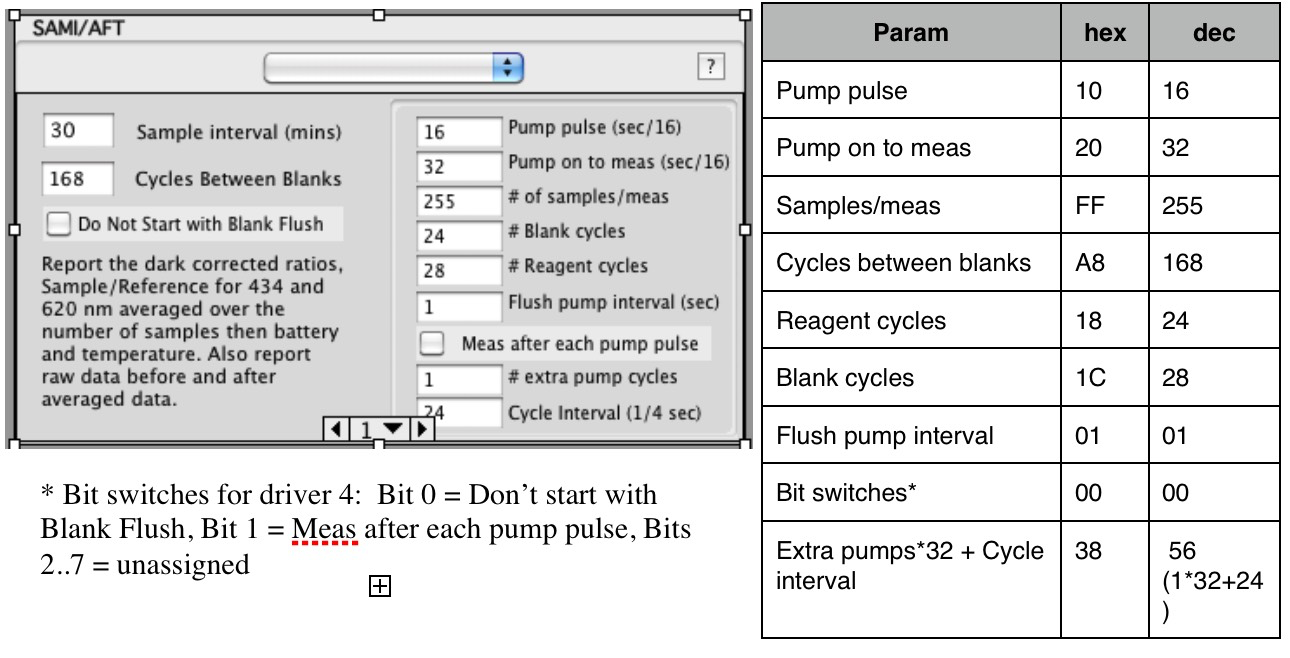
\includegraphics[width=\textwidth]{figs/Image1.png}


\subsection*{Command Format}

\begin{itemize}
\item
  Command format: one letter followed by a number of arguments as hex
  numbers and ending with carriage return (\cmdfont{CR}).
\item
  Args may be separated by Space, Tab, comma, '/' or ':' the first
  separator may be omitted. For example "T 03/05/29 5 12:30:06" is
  equivalent to "T3 5 29,5,12 30 06"
\item
  123 is equivalent to 000123 if a long word is expected 0123 if a word
  or 23 if a byte.
\item
  If more bytes are entered than the command uses the left most (first
  entered) bytes are ignored. For example, a command that takes a byte
  will read \cmdfont{1A2B} as \cmdfont{2B}.
\item
  Arguments are represented as follows:
\end{itemize}

\begin{quote}
(\cmdfont{B}) One byte (\cmdfont{S}) 12 bits (\cmdfont{W}) 2 bytes (\cmdfont{L}) 3 bytes (\cmdfont{E}) 4 bytes (\cmdfont{X}) don't
care, () none, (\cmdfont{N}) nibble

\{\} indicates return expected using above while \{R\} means returns
record

(\cmdfont{5A}) sending \cmdfont{5A} enables a variant of the commands normal function
\end{quote}

\begin{itemize}
\item
  Arguments in {[} {]} are optional. Typically these optional arguments
  are present for a ``write'' to the \instType{} and omitted if the user wants
  to ``read'' from the \instType{}.

\item
  No backspace or delete support for cmds sent - type non-hex arg with
  \cmdfont{CR} to abort.

\item
  Results (reads) are returned as space separated hex and terminated
  with \cmdfont{CR}.

\item
  Commands that are illegal or malformed return \cmdfont{?}, error code in hex
  followed by return.

\item
  Any input returns \cmdfont{!} if a command or process is running.

\item
  Echo is off by default. Echo off suppresses prompts and error text.
  Use \cmdfont{I} command to enable echo.
\end{itemize}


\subsubsection*{Command List}

%C run blank
{\cmdfont{\textbf{C}} ()\{R\} Run Blank cycle on SAMI-\dioxide{}}
\begin{quote}
	() - no argument required\\
	\{R\} - returns a data record\\
	A valid configuration is required. If \instType{} erased then error returned.\\
	Returns (and if running writes) a data record.\\
\end{quote}

%D dump memory
{\cmdfont{\textbf{D}} (W,{[}B{]},{[}W{]}) \{memory stream\} Dump Memory}
\begin{quote}
	(W - arg1) is number of pages beginning from page 0.\\
	{[}B - arg2 {]} - optional format switch 0 for binary, 1 for hex
	(default is binary)\\
	{[}W - arg3 {]} - optional start page\\
	B - bit 0=1 send as hex return after page, bit 0=0 send as binary\\
	Begins streaming memory with first data record.\\
\end{quote}

%E erase
{\cmdfont{\textbf{E}} ({[}B{]})\{W\} Erase}
\begin{quote}
	() - no argument erases \instType{} memory\\
	(5A) - for safety erase all of memory and clear ram vars.\\
	\{W\} - returns the first unerased page or 8000 if all are erased\\
	Erase shuts down all activity including time keeping but allows serial
	commands.\\
	Stops real time clock\\
\end{quote}

%F status ticks
{\cmdfont{\textbf{F}} (B)() Status ticks on/off \& special cmd mode}
\begin{quote}
	(5A) - turns ticks off -turn off 1/sec status from \instType{} Enable Debug
	commands\\
	(55) - turns on optional commands (see section below)\\
	(any other byte) - turns ticks on and disables optional commands\\
\end{quote}

%G open flash
{\cmdfont{\textbf{G}} ({[}B{]})() Open flash and start recording}
\begin{quote}
	Starts real time clock if it is not running
	Clears n\_drec number of records, n\_erec number of error records.
	n-bytes Number of bytes stored - Is set to the start of the page after
	the last un-erased page.
	Restarting without erase is supported.\\
\end{quote}

%H read ADC channel
{\cmdfont{\textbf{H}} (N)\{S\} Read one adc channel}
\begin{quote}
	(N) - Channel 0..7 or\\
	\{S\} - returns in Hex ADC count Voltage = (S/4096)*5.00V\\
	0 - Photo Reference, gated in firmware so not useful\\
	1 - Photo Signal, gated in firmware so not useful\\
	2 - Battery if 12V is enabled else 0 V= count/4096*5V*3 Volts\\
	3 - Thermistor\\
	4 - 3rd Party input J6 pin8 - 5V full scale\\
	5 - 3rd Party input J6 pin8 - 5V full scale\\
	6 - 3rd Party input J6 pin8 - 5V full scale\\
	7 - 3rd Party input J6 pin8 - Photo diode amplified current input\\
	
	\underline{Special}
	
	If arg $\geq$\,80 turn on 12\,V and read Batt, therm, 5\,V in 1, 5\,V
	in 2, 5\,V in 3, photodiode restore 12\,V
	
	Returns \{S S S S S S\}\\
\end{quote}

%I immediate read
{\cmdfont{\textbf{I}} ({[}B{]})\{B\} Immediate read status sw \& bus}
\begin{quote}
	arg switches\\
	Bit 0 Pump on\\
	Bit 1 Valve on\\
	Bit 2 12V on\\
	Bit 3 Reserved - was Battery sense enable\\
	Bit 4 debug LED off\\
	Bit 5 echo off\\
	Bit 6 Reserved\\
	Bit 7 Reserved\\
	Return Switches \{B\} as in arg\\
\end{quote}

%J invoke loader
{\cmdfont{\textbf{J}} (B) invokes loader returns nothing, used to load firmware
after erase}
\begin{quote}
	(5A) - branch to loader\\
	(5C) - Erase Board Type and SN 128 Bytes in microcontroller flash\\
\end{quote}

%L load or read config
\label{sec:Lcommand}
{\cmdfont{\textbf{L}} ({[}5A{]})\{ConfigString\} Load or Read Config + UserText}
\begin{quote}
	-\/- Read or load a string. Consisting of Configuration string (+ fill to
	256 bytes) + UserText\\
	() No argument gets configuration string from board.\\
	(5A) - start 4 byte timer at zero and wait for \cmdfont{CR} from board
	After receiving carriage return, send load data as packed hex with no
	separator.\\
	First non-hex non-return character causes abort of load.\\
	Either a null between byte 256 and 512 or 512 bytes is a valid\\
	termination. Any non hex is an error.\\
	Returns 2-byte checksum read from flash after write.\\
	Successful load starts real time clock. Erase or reset stops clock\\
\end{quote}

%M measure LEDs 
{\cmdfont{\textbf{M}} ({[}B{]})\{S,S,S,S,S,S\} Measure LEDs w/o pumping}
\begin{quote}
	Read the ADC values no pump cycle\\
	Arg default = FF (read all)\\
	Bits enable sending of data below bit 2..7 - blue ref...dark signal\\
	Returns \{S\} in same order as below\\
	bit2 - Dark ref\\
	bit3 - Dark signal\\
	bit4 - LED1 ref\\
	bit5 - LED1 signal\\
	bit6 - LED2 ref\\
	bit7 - LED2 signal\\
\end{quote}

%N -compare
{\cmdfont{\textbf{N}} ( {[}B{]} B W W) }
\begin{quote}
	Compare or write a byte value to a range of memory W as page count\\
	Verify N(byte value, word Start\_page, word count\_pages) Return (0 if
	true, first failed page if false)\\
	Write N(\$5A, byte value, word Start\_page, word count\_pages)\\
	Progress reporting\\
	Returns hight byte of page +1 for each page started then XX last page
	address where XX=00 for good FF for fail\\
	(Should fix this, should be page started then 2 byte end address and 00
	or FF)\\
\end{quote}

%O readwrite port
{\cmdfont{\textbf{O}} ({[}B{]}) \{B\} Read or write port A - set bits enable power
out function}s
\begin{quote}
	() - no arg is `read' with \{B\} returned as described below\\
	(B) - arg writes to port A to turn on/off power out as below
	
	Bit0 - 12\,V\\
	Bit1 - Valve - J4 pin6\\
	Bit2 - Pump - J4 pin7\\
	Bit3 - 3rd party power J5 pin 6\\
	Bit4 - 3rd party power J5 pin 5\\
	Bit5 - 3rd party power J5 pin 4\\
	Bit6 - Select 12\,V for 3rd party power\\
	Bit7 - Select Battery for 3rd party power\\
	Note that if both bit 6 and 7 are set, bit 7 is cleared - 12\,V is
	selected\\
\end{quote}

%P - pump valve
{\cmdfont{\textbf{P}} ({[}B{]},{[}B{]}) Pump and valve powering}
\begin{quote}
	() - no argument pump and valve off\\
	(B1) - one arg set pump and valve on or off\\
	(B1,B2) - 2 args set on or off and restore after arg2 1/8 seconds\\
	B1 - bit 0 turns pump on, bit 1 turns valve on\\
	B2 - time to hold state of B1 before returning to original state (1/8's
	sec)\\
	Turns on 12\,V supply if required and restores to original state\\
	Return Null just carriage return after time out - single threaded\\
\end{quote}

{\textbf{Q} (5A)() Close flash and stop recording.}\\

%R run sample
{\cmdfont{\textbf{R}} ({[}B{]})(R) Run sample cycle on device}
\begin{quote}
	Arg Slot Default device is \instType{} - 0 slot1..3, PMI is 4\\
	Arg set bit 3 returns test error/info rec\\
	Arg bit 2 selects error/info record\\
	A valid configuration is required. If erased then error.\\
	Returns (and if running writes) a data record\\
\end{quote}

%S - status report
{\cmdfont{\textbf{S}} ({[}B{]})\{: E,W,L,L,L,W,W\} Ask for status from \instType{} (note
this is auto sent when RTS is high)}
\begin{quote}
	(B) If arg=0 (default) returns \cmdfont{:} followed by \cmdfont{:}\\
	\{E\} time in seconds since \cmdfont{L} command - Cleared by Erase\\
	\{W\} statusflags - Cleared by Erase, defined here:
\end{quote}

\begin{quote}
	bit 0 Clock started\\
	bit 1 Recording started\\
	bit 2 Recording ended on time\\
	bit 3 Recording ended memory full\\
	bit 4 Recording ended due to error, failure, or user stopped\\
	bit 5 Data downloded\\
	bit 6 Flash Open\\
	bit 7 *Low or no battery before start 256*t\_pmi seconds - fatal\\
	bit 8 Battery low on measure cycle - fatal\\
	bit 9 Battery low on blank cycle - fatal\\
	bit 10 *Battery low on external device cycle - fatal\\
	bit 11 *External device 1 fault - fatal for device shut it down\\
	bit 12 *External device 2 fault - fatal for device shut it down\\
	bit 13 *External device 3 fault - fatal for device shut it down\\
	bit 14 Erased\\
	bit 15 Power on flags not valid
	
	( * Not yet implemented )\\
\end{quote}

\begin{quote}
	\{L\} - n\_rec (3) number of data records - Cleared by Erase\\
	\{L\} - n\_erec (3) number of error records - Cleared by Erase\\
	\{L\} - n\_bytes (3) Number of bytes stored including config and user
	text as full pages - Cleared by Erase\\
	If arg=1 returns Name(16) SN(4) FirmwareVer(4) \instType{} board version(2)
	\instType{} board Config(2) Cal(24) Cksum(1)\\
	If arg=2 returns 128 bit microcontroller flash Name(16) SN(4)
	calibration TBD Checksum(1)
\end{quote}


\subsubsection*{Commands turned on by \cmdfont{F55} command }

\cmdfont{\textbf{@}} ({[}X{]},{[}X{]},{[}X{]}...)(T) Test the command parser
\begin{quote}
	Debug tool only works if echo is on.\\
	Reports in text the number and value of args.\\
\end{quote}

\cmdfont{\textbf{A}} (X)(T) List all commands
\begin{quote}
	Debug tool only works if echo is on.\\
	Lists all the commands.\\
\end{quote}

\cmdfont{\textbf{B}} ( )(S) Battery Voltage
\begin{quote}
	S the battery voltage 12\,V must be enabled $V_bat = Arg * 5 * 3 / 4096$\\
\end{quote}

\cmdfont{\textbf{T}} () (s) Thermistor Voltage
\begin{quote}
	$V= 4096 * Thermistor Res / (Thermistor Res + 17400)$
\end{quote}


\subsubsection*{Debug tools hidden - enabled by \cmdfont{F5A}}

\cmdfont{\textbf{Z}} (W)( ) Set breakpoint

\cmdfont{\textbf{\^{}C}} Break to debugger

\cmdfont{\textbf{\^{}T}} Show current program address and reg.


\subsubsection*{Extra debug commands for now}

\cmdfont{\textbf{K}} Send error \cmdfont{CF} with 2 extra bytes \&h0201

\cmdfont{\textbf{V}} No arg send 'Hello World' out secondary port and echo for 10 sec then
return 'Done'

\cmdfont{\textbf{V}} Any arg send 'Hello World' out serial port and return 0 if all\\
characters echo - for tester

\cmdfont{\textbf{W}} Return status word, MFG code, etc.

\cmdfont{\textbf{X}} Sleep for ever but wake every 8 sec and send time - reset to exit

\cmdfont{\textbf{Y}} Show time, internal flags, wake counter


\subsubsection*{Notes}

While DTR is present on the serial port command mode is maintained and 5\,V power is on. 12\,V power is off by default but can be turned on with \cmdfont{I} or \cmdfont{O} command.

12\,V power will cycle on and off as needed to run pump or valve.

\subsubsection*{*** Command Error Codes ***}
\begin{quote}
	\cmdfont{00} Wrong Number of Arguments\\
	\cmdfont{01} Command Not Implemented\\
	\cmdfont{02} Invalid Arguments\\
	\cmdfont{03} Command Buffer Overflow\\
	\cmdfont{04} Invalid Command Enter A return for a list of commands\\
	\cmdfont{05} Error in config data\\
	\cmdfont{06} \textgreater{} 2000 pages\\
	\cmdfont{07} Invalid Configuration\\
	\cmdfont{08} Bad Key\\
	\cmdfont{09} Flash is Open\\
	\cmdfont{0A} Flash is Not Open\\
	\cmdfont{0B} Too Many Arguments\\
	\cmdfont{0C} Too Few Arguments\\
	\cmdfont{0D} Memory Full\\
    	\cmdfont{0E} Not Valid With Echo Off\\
	\cmdfont{0F} Unimplemented Extenstion Index in Configuration\\
	\cmdfont{10} Flash Data not erased\\
	\cmdfont{11} Invalid Arguments
\end{quote}

\clearpage

\subsection*{Error conditions}

No battery - If main battery without load at wake from sleep is below
Vmin.

\instType{} counts no battery event and schedules next wake for measurement.

Note that \instType{} does not attempt to write Flash memory on backup battery.

If 2 byte no battery count overflows \instType{} shuts down completely.

If \instType{} awakes to find battery restored it writes an error record with
counts and time and resumes normal operation.

Battery fail - if \instType{} tries to power up analog, pump, valve, or
external device and battery falls below Vmin:
\begin{itemize}
	\item[]
	write an error record
	
	\item[]
	close Flash page
	
	\item[]
	shutdown completely until handshake from host.
\end{itemize}